%!TEX root = main.tex


\section{Variables and Probability Models}\label{sec:vague_variables}

\subsection{Semantics of observed and unobserved variables}\label{sec:variables}

We are interested in constructing \emph{probabilistic models} which explain some part of the world. In a model, variables play the role of ``pointing to the parts of the world the model is explaining''. Both observed an unobserved variables play important roles in causal modelling and we think it is worth clarifying what variables of either type refer to. Ultimately, our interpretation is largely the standard one: a probabilistic model is associated with an experiment or measurement procedure that yields values in a well-defined set. Observable variables are obtained by applying well-defined functions to the result of this total measurement. We explain how we can use a richer sample space that includes unobserved variables. Unobserved variables are formally modelled in exactly the same way as observed variables, but unlike observed variables we don't offer a standard interpretation of unobserved variables. 

Consider Newton's second law in the form $\proc{F}=\proc{MA}$ as a simple example of a model that relates variables $\proc{F}$, $\proc{M}$ and $\proc{A}$. As \citet{feynman_feynman_1979} noted, this law is incomplete -- in order to understand it, we must bring some pre-existing understanding of force, mass and acceleration as independent things. Furthermore, the nature of this knowledge is somewhat perculiar. Acknowledging that physicists happen to know a great deal about determining the forces on an object, it remains true that in order to actually say what the net force on a real object is, even a highly knowledgeable physicist will still have to go and do some measurements, and the result of such measurements will be a vector representing the net forces on that object.

This suggests that we can think about ``force'' $\proc{F}$ (or mass or acceleration) as a kind of procedure that we apply to a particular real world object and which returns a mathematical object (in this case, a vector). We will call $\proc{F}$ a \emph{procedure}. Our view of $\proc{F}$ is akin to \citet{menger_random_2003}'s notion of variables as ``consistent classes of quantities'' that consist of pairing between real-world objects and quantities of some type. Force $\proc{F}$ itself is not a well-defined mathematical thing, as measurement procedures are not mathematically well-defined. At the same time, the set of values it may yield \emph{are} well-defined mathematical things.

We will assume that any procedure will eventually yield an unambiguous value in a defined mathematical set. No actual procedure can be guaranteed to have this property -- any apparatus, however robust, could suffer catastrophic failure -- but we assume that we can study procedures reliable enough that we don't lose much by making this assumption. This assumption allows us to say a procedure $\proc{B}$ yields values in $B$. $\proc{B}\bowtie x$ is the proposition that $\proc{B}$, when completed, yields the value $x\in B$, and by assumption exactly one of these propositions is true. For $A\subset B$, $\proc{B}\bowtie A$ is the proposition $\lor_{x\in A} \proc{B}\bowtie x$. Two procedures $\proc{B}$ and $\proc{C}$ are the same if $\proc{B}\bowtie x\iff \proc{C}\bowtie x$ for all $x\in B$. 

The notion of ``yielding values'' allows us to define an operation akin to function composition. If I have a procedure $\proc{B}$ that takes values in some set $B$, and a function $f:B\to C$, define the ``composition'' $f\circ \proc{B}$ to be the procedure $\proc{C}$ that yields $f(x)$ whenever $\proc{B}$ yields $x$. For example, $\proc{MA}$ is the composition of $h:(x,y)\mapsto xy$ with the procedure $(\proc{M},\proc{A})$ that yields the mass and acceleration of the same object. Composition is associative - for all $x\in B$: 

\begin{align}
	(g\circ f)\circ\proc{B}\text{ yields } x &\iff B\text{ yields } (g\circ f)^{-1}(x) \\
	&\iff B\text{ yields } f^{-1}(g^{-1}(x))\\
	&\iff f\circ B \text{ yields } g^{-1}(x)\\
	&\iff g\circ(f\circ B)\text{ yields } x
\end{align}


One might whether there is also some kind of ``append'' operation that takes a standalone $\proc{M}$ and a standalone $\proc{A}$ and returns a procedure $(\proc{M},\proc{A})$. Unlike function composition, this would be an operation that acts on two procedures rather than a procedure and a function. Rather than attempt to define any operation of this type, we simply assume that somehow a procedure has been devised that measures everything of interest, which we will call $\proc{S}$ which takes values in $\Psi$. We assume $\proc{S}$ is such that any procedure of interest can be written as $f\circ \proc{S}$ for some $f$.

For the model $\proc{F}=\proc{MA}$, for example, we could assume $\proc{F}=f\circ \proc{S}$ for some $f$ and $(\proc{M},\proc{A})=g\circ \proc{S}$ for some $g$. In this case, we can get $\proc{MA}=h\circ(\proc{M},\proc{A})=(h\circ g)\circ\proc{S}$. Note that each procedure is associated with a unique function with domain $\Psi$.

Thus far, $\Psi$ is a ``sample space'' that only contains observable variables. To include unobserved variables, we posit a richer sample space $\Omega$ such that the measurement $\proc{S}$ determines an element of some partition of $\Omega$ rather than an element of $\Omega$ itself. Then, by analogy to procedures defined with respect to $\proc{S}$, we identify variables in general with measurable functions defined on the domain $\Omega$. 

Specifically, suppose $\proc{S}$ takes values in $\Psi$. Then we can propose a sample space $\Omega$ such that $|\Omega|\geq |\Psi|$ and a surjective function $\RV{S}:\Omega\to \Psi$ associated with $\proc{S}$. We connect $\Omega$, $\RV{S}$ and $\proc{S}$ with the notion of \emph{consistency with obseravation}:

\begin{align}
 &\omega\in \Omega\text{ is \emph{consistent with observation} iff the result yielded by }\proc{S}\text{ is equal to }\RV{S}(\omega)\label{def:observable}
\end{align}

Thus the procedure $\proc{S}$ eventually restricts the observationally consistent elements of $\Omega$. If $\proc{S}$ yield the result $s$, then the consistent values of $\Omega$ will be $\RV{S}^{-1}(s)$.

One thing to note in this setup is that two different sets of measurement outcomes $\Psi$ and $\Psi'$ entail a different mesurement procedures $\proc{S}$ and $\proc{S}'$, but different sample spaces $\Omega$ and $\Omega'$ may be used to model a single procedure $\proc{S}$. We will sometimes consider different models of the same observable procedures.

As far as we know, distinguishing variables from procedures is somewhat nonstandard, but it is a useful distinction to make. While they may not be explicitly distinguished, both variables and procedures are often discussed in statistical texts. For example, \citet{pearl_causality:_2009} offers the following two, purportedly equivalent, definitions of variables:
\begin{quote}
By a \emph{variable} we will mean an attribute, measurement or inquiry that may take on one of several possible outcomes, or values, from a specified domain. If we have beliefs (i.e., probabilities) attached to the possible values that a variable may attain, we will call that variable a random variable.
\end{quote}

\begin{quote}
This is a minor generalization of the textbook definition, according to which a random variable is a mapping from the sample space (e.g., the set of elementary events) to the real line. In our definition, the mapping is from the sample space to any set of objects called ``values,'' which may or may not be ordered.
\end{quote}

Our view is that the first definition is a definition of a procedure, while the second is a definition of a variable. Variables model procedures, but they are not the same thing. We can establish this by noting that, under our definition, every procedure of interest -- that is, all procedures that can be written $f\circ \proc{S}$ for some $f$ -- is modeled by a variable, but there may be variables defined on $\Omega$ that do not factorise through $\proc{S}$, and these variables do not model procedures.

\subsection{Events}

To recap, we have a procedure $\proc{S}$ yielding values in $\Psi$ that measures everything we are interested in, a sample space $\Omega$ and a function $\RV{S}$ that models $\proc{S}$ in the sense of Definition \ref{def:observable}. We assume also that $\Psi$ has a $\sigma$-algebra $\sigalg{E}$ (this may be the power set of $\Psi$, as measurement procedures are typically limited to finite precision). $\Omega$ is equipped with a $\sigma$-algebra $\sigalg{F}$ such that $\sigma(\RV{S})\subset \sigalg{F}$. If a procedure $\proc{X}=f\circ \RV{S}$ then we define $\RV{X}:\Omega\to X$ by $\RV{X}:=f\circ\RV{S}$.

If a particular procedure $\proc{X}=f\circ \proc{S}$ eventually yields a value $x$, then the values of $\Omega$ consistent with observation must be a subset of $\RV{X}^{-1}(x)$. We define an \emph{event} $\RV{X}\bowtie x:\equiv \RV{X}^{-1}(x)$, which we read ``the event that $\RV{X}$ yields x''. An event $\RV{X}\bowtie x$ occurs if the consistent values of $\Omega$ are a subset of $\RV{X}\bowtie x$, thus ``the event that $\RV{X}$ yields x occurs$\equiv \proc{X}$ yields $x$''. The definition of events applies to all types of variables, not just observables, but we only provide an interpretation of events ``occurring'' when the variable $\RV{X}$ is associated with some $\proc{X}$.

For measurable $A\in \sigalg{X}$, $\RV{X}\bowtie A=\bigcup_{x\in A} \RV{X}\bowtie x$. 

Given $\RV{Y}:\Omega\to X$, we can define an append operation for variables: $(\RV{X},\RV{Y}):=\omega\mapsto (\RV{X}(\omega),\RV{Y}(\omega))$. $(\RV{X},\RV{Y})$ has the property that $(\RV{X},\RV{Y})\bowtie (x,y)= \RV{X}\bowtie x\cap \RV{Y}\bowtie y$, which supports the interpretation of $(\RV{X},\RV{Y})$ as the values yielded by $\RV{X}$ and $\RV{Y}$ together.

It is common to use the symbol ``$=$'' instead of ``$\bowtie$'', but we want to avoid this because $\RV{Y}=y$ already has a meaning, namely that $\RV{Y}$ is a constant function everywhere equal to $y$.

\subsection{Probabilistic models for causal inference}

We have a ``skeletal model'' process $\proc{S}$, a sample space $(\Omega,\sigalg{F})$ and a collection of \emph{variables}, which we write with the sans serif font: $\RV{X},\RV{Y}_i$. The process $\proc{S}$ is related to the model $\Omega$ and the observable variables via the notion of \emph{consistency with observation}. To this skeleton, we want to add a model that relates variables probabilistically. Without delving into it too deeply, such a model can be thought to be something like a quantitative forecast of the results eventually yielded by $\proc{S}$.

For causal inference, we need to modify the standard approach to constructing probability models on a sample space $(\Omega,\sigalg{F})$ to allow for \emph{gaps} in our model. \citet{hajek_what_2003} defines \emph{probability gaps} as propositions that do not have a probability assigned to them. Probability gaps arise particularly often when some variables represent choices. Because we use the probability model to make choices, we typically only work out what choice we're going to make after we settle on all other important aspects of the model. Another area we sometimes see probability gaps is for prior probabilities.

For this example, we will assume that the reader is familiar enough with marginal probabilities, conditional probabilities and causal models to follow along. We will offer more careful definitions of terms subsequently.

Suppose we have a causal Bayesian network $(\prob{P}^{\RV{XYZ}},\mathcal{G})$ where $\RV{X}:\Omega\to X$, $\RV{Y}:\Omega\to Y$ and $\RV{Z}:\Omega\to Z$ are variables, $\prob{P}^{\RV{XYZ}}$ is a probability measure on $X\times Y\times Z$ that we call ``a probability model of $(\RV{X},\RV{Y},\RV{Z})$'' and $\mathcal{G}$ is a Directed Acyclic Graph whose vertices we identify with $\RV{X}$, $\RV{Y}$ and $\RV{Z}$ that contains the edges $\RV{X}\longrightarrowRHD \RV{Y}$ and $\RV{X}\longleftarrowRHD \RV{Z} \longrightarrowRHD \RV{Y}$. ``Setting $\RV{X}$ to $x$'' is an operation that takes as inputs $\prob{P}^{\RV{XYZ}}$, $\mathcal{G}$ and some $x\in X$ and returns a new probability measure $\prob{P}_x^{\RV{XYZ}}$ on $X\times Y\times Z$ given by \citep[page ~24]{pearl_causality:_2009}:
\begin{align}
	\prob{P}^{\RV{XYZ}}_{x}(x',y,z)=\prob{P}^{\RV{Y|XZ}}(y|x,z)\prob{P}^{\RV{Z}}(z)\llbracket x=x' \rrbracket\label{eq:truncated_fac}
\end{align}

Equation \ref{eq:truncated_fac} embodies three assumptions about a model of the operation of ``setting $\RV{X}$ to $x$''. First, such a model must assign probability 1 to the proposition that $\RV{X}$ yields $x$. Second, such a model must assign the same marginal probability distribution to $\RV{Z}$ as the input distribution; $\prob{P}^{\RV{Z}}=\prob{P}_{x}^{\RV{Z}}$. Finally, our model must also assign the same conditional probability to $\RV{Y}$ given $\RV{X}$ and $\RV{Z}$; $\prob{P}^{\RV{Y}|\RV{XZ}}=\prob{P}_x^{\RV{Y}|\RV{XZ}}$.

Notice that the map $x\mapsto \prob{P}^{\RV{XYZ}}_x$ itself has the type of a conditional probability - that is, it takes some $x\in X$ and returns a probability distribution over $(\RV{X},\RV{Y},\RV{Z})$. In fact, a popular notation for this map suggests that it is a conditional probability of sorts: $\prob{P}^{\RV{XYZ}|do(\RV{X}=x)}$. Suppose that this actually is a conditional probability. That is, suppose $\RV{X}$ is an observable associated with $\proc{X}$ and I have some choice available that I believe can dictate the value yielded by $\proc{X}$ (alternatively, I can dictate that $\RV{X}\bowtie x$ occurs for any $x\in X$), and furthermore I have some $\proc{U}$ (modeled by $\RV{U}$), taking values in $X$, that yields whatever choice I end up making. Then I can define a probabilisitic model $\prob{Q}^{\RV{XYZ}|\RV{U}}:=x\mapsto \prob{P}^{\RV{XYZ}}_x$.

Now, the result yielded by $\proc{U}$ is a matter of choice, and I may be perfectly capable of making this choice without specifying a probability distribution $\prob{Q}^{\RV{U}}$. If so, I can leave $\prob{Q}^{\RV{U}}$ as a \emph{probability gap}, and $\prob{Q}^{\RV{XYZ}|\RV{U}}$ is thus a \emph{probability model with a gap}.

There are a few features of $\prob{Q}^{\RV{XYZ}|\RV{U}}$ we want to point out. Firstly, $\prob{Q}^{\RV{XYZ}|\RV{U}}$ should be unique, but Equation \ref{eq:truncated_fac} does not necessarily yield a unique $\prob{P}^{\RV{XYZ}}_{x}$ for each $x$. If there are measure zero sets in the range of $(\RV{X},\RV{Z})$ then $\prob{P}^{\RV{Y|XZ}}$ can be chosen arbitrarily on these sets, and because these do not necessarily correspond to zero measure sets in the range of $\RV{Z}$, different choices can lead to different versions of $\prob{P}^{\RV{XYZ}}_{x}$.

Secondly, $\prob{Q}^{\RV{XYZ}|\RV{U}}$ should be valid, but Equation \ref{eq:truncated_fac} does not always yield a valid probability model. For example, if $\RV{X}=\RV{Z}$ -- which is to say, $\RV{X}$ and $\RV{Z}$ are the same function on $\Omega$ -- then any probability model must assign probability 1 to the event $(\RV{X},\RV{Z})\bowtie \{(x,x)|x\in X\}$. However, this cannot be done in accordance with Equation \ref{eq:truncated_fac} for all $x\in X$ if $|X|\geq 2$ because for $x\neq x'\in X$, $\prob{P}_x^{\RV{X}}\neq \prob{P}_{x'}^{\RV{X}}$ while $\prob{P}_x^{\RV{Z}}=\prob{P}_{x'}^{\RV{Z}}$. In addition, $\prob{Q}^{\RV{XYZ}|\RV{U}}$ should be extendable to a valid $\prob{Q}_\alpha^{\RV{XYZU}}$ for every $\prob{Q}_\alpha^{\RV{U}}$ that ``fills the gap''.

To construct probability models with gaps in them, we need to address these two issues -- uniqueness and valid extendability.

\todo[inline]{The following is an extension of the point (2), I think it's interesting but also a complication. Not quite sure where to put it}

The example of $\RV{X}=\RV{A}$ might seem absurd. Consider instead $\RV{Z}=(\RV{H},\RV{W})$, representing the height in metres and weight in kilograms of a particular person, and $\RV{X}$ represents their body mass index, which is to say $\RV{X}=\frac{\RV{W}}{\RV{H}^2}$ (not that in both cases we are using ``$=$'', which means these variables are \emph{equal as functions}, not that they \emph{yield the same result with probability 1}, which would involve the symbol ``$\bowtie$''). A causal graph with exactly these variables and arrows analogous to ours appears in \citet{shahar_association_2009}. However, generally there is no $\prob{P}_x^{\RV{XHW}}$ that satisfies both $\RV{X}\bowtie \frac{\RV{W}}{\RV{H}^2}$ with probability 1 and Equation \ref{eq:truncated_fac}. This is true, for example, whenever $\prob{P}^{\RV{X}}$ has support at more than one point.

\subsection{Probability models}

Define $\RV{I}:\Omega\to \Omega$ as the identity function $\omega\mapsto \omega$. A \emph{standard probability model} on $(\Omega,\sigalg{F})$ is a probability distribution $\prob{P}^{\RV{I}}$ on $(\Omega,\sigalg{F})$.

Given a standard probability model $\prob{P}^{\RV{I}}$ and $\RV{X}:\Omega\to X$, the probability that $\RV{X}\bowtie A$ for $A\in\sigalg{X}$ is defined as $\prob{P}^{\RV{X}}(A):=\prob{P}^{\RV{I}}(\RV{X}\bowtie A)$. $\prob{P}^{\RV{X}}$ is known as the pushforward of $\prob{P}^{\RV{I}}$ via $\RV{X}$. We use the convention that the same base letter appearing in $\prob{P}^{\RV{I}}$ and $\prob{P}^{\RV{X}}$ indicates $\prob{P}^{\RV{X}}$ is a pushforward of $\prob{P}^{\RV{I}}$. 

Any \emph{sample space-valid} probability distribution $\prob{Q}^{\RV{X}}$ is the pushforward of some $\prob{Q}^{\RV{I}}$.

\subsection{Validity of probability models with gaps}\label{sec:validity_of_gapprob}

A conditional probability can be considered to be a model with a probability gap. For example, suppose I have two variables $\RV{X}:\Omega\to X$ and $\RV{Y}:\Omega\to Y$, and I have some known $\prob{P}^{\RV{Y}|\RV{X}}$ but ``the probability of $\RV{X}$'' is a probability gap. In this case, I can define a map that takes an arbitrary $\prob{P}_\alpha^{\RV{X}}$ and returns $\prob{P}^{\RV{XY}}_\alpha:=\prob{P}_\alpha^{\RV{X}}\odot \prob{P}^{\RV{Y}|\RV{X}}$ (definition \ref{def:copyproduct}). Thus $\prob{P}^{\RV{Y}|\RV{X}}$ is an example of a probability model with a gap.

We want models with probability gaps that are \emph{validly extendable}: given a valid proposed model that fills the probability gap, we get a unique, sample space-valid probability distribution. To examine this issue, we will firstly define the copy-product between two Markov kernels. This is the standard operation we use to extend conditional probabilities.

\begin{definition}[Copy-product]\label{def:copyproduct}
Given two Markov kernels $\kernel{K}:X\kto Y$ and $\kernel{L}:Y\times X\kto Z$, define the copy-product $\kernel{K}\odot\kernel{L}$ as
\begin{align}
	\kernel{K}\odot\kernel{L}:&= \text{copy}_X(\kernel{K}\otimes \text{Id}_X)(\text{copy}_Y\otimes\text{Id}_X )(\text{Id}_Y \otimes \kernel{L})\\
							&= \tikzfig{copy_product}\\
							&\iff\\
	(\kernel{K}\odot\kernel{L})(A\times B|x) &= \int_A\kernel{L}(B|y)\kernel{K}(dy|x)
\end{align}
\end{definition}

We want extensions of conditional probabilities via $\odot$ to be sample space-valid, but this is not true for arbitrary conditional probabilities $\prob{P}^{\RV{Y}|\RV{X}}$ yield invalid extensions $\prob{P}_\alpha^{\RV{XY}}$ from this operation. For example, suppose $X=Y$ and $\RV{X}=\RV{Y}$. Then given $x\neq x'\in X$ such that $\prob{P}^{\RV{Y}|\RV{X}}(x|x')=a>0$, we could choose $\prob{P}_\alpha^{\RV{X}}(\{x'\})=1$ and then $\prob{P}_\alpha^{\RV{XY}}(\{(x',x)\})=a>0$ also. To begin with, it is absurd to assign nonzero probability to the proposition $\RV{X}\not\bowtie\RV{X}$. Furthermore for every probability model $\prob{Q}^{\RV{I}}\in \Delta(\Omega)$,
\begin{align}
\prob{Q}^{\RV{XY}}(\{(x,x')\})&=\prob{Q}^{\RV{I}}(\RV{X}^{-1}(x)\cap\RV{X}^{-1}(x'))\\
&= \llbracket x=x' \rrbracket
\end{align}
Thus $\prob{P}_\alpha^{\RV{XY}}$ is not sample space-valid.

We already have a validity criterion for probability distributions. We propose a slightly different validity criterion for conditional probabilities.

\begin{definition}[Valid conditional probability]\label{def:valid_conditional_prob}
Given $(\Omega,\sigalg{F})$, $\RV{X}:\Omega\to X$, $\RV{Y}:\Omega\to Y$ a \emph{valid conditional probability} $\prob{P}^{\RV{Y}|\RV{X}}$ is a Markov kernel $X\kto Y$ such that it assigns probability 0 to contradictions:
\begin{align}
	\forall A\in \sigalg{Y}, x\in X: \RV{X}^{-1}(x)\cap \RV{Y}^{-1}(A) = \emptyset \implies \left(\prob{P}^{\RV{Y}|\RV{X}}(A|x) = 0\right) \lor \left(\RV{X}^{-1}(x) = \emptyset\right)
\end{align}
\end{definition}

The requirement that a conditional probability be valid means that if the variables themselves rule out certain values, then these values must be assigned zero probability. For example, $\prob{P}^{\RV{X}|\RV{X}}(x'|x)=0$ if $x'\neq x$. In addition, it implies that $\prob{P}^{\RV{X}|\RV{X}}=1$. If we start with a standard probability model and derive conditional probabilities from it, then validity holds up to a set of measure zero. In our case, valid conditional probabilities guarantee that we can extend the conditional probability to a standard probability model.

\begin{theorem}[Agreement of validity criteria for probability distributions]\label{th:valid_agree}
Given $\RV{X}:\Omega\to X$ with $(\Omega,\sigalg{F})$ and $(X,\sigalg{X})$ standard measurable, a probability $\prob{P}^{\RV{X}}$ is sample space-valid if and only if the conditional probability $\prob{P}^{\RV{X}|*}:=*\mapsto \prob{P}^{\RV{X}}$ is valid.
\end{theorem}

\begin{proof}
$*^{-1}(*)=\Omega$ necessarily. Thus validity of $\prob{P}^{\RV{X}|*}$ means 

\begin{align}
	\forall A\in \sigalg{X}: \RV{X}^{-1}(A)=\emptyset \implies \prob{P}^{\RV{X}|*}(A|*)&=0\\
	&= \prob{P}^{\RV{X}}(A)\label{eq:nec_and_suff}
\end{align}

If: We refer to \citet{ershov_extension_1975} Theorem 2.5 for the proof that Equation \ref{eq:nec_and_suff} is necessary and sufficient for the existence of $\prob{P}^{\RV{I}}$ such that $\prob{P}^{\RV{I}}(\RV{X}^{-1}(A))=\prob{P}^{\RV{X}}(A)$ for all $A\in \sigalg{X}$ when $(\Omega,\sigalg{F})$ and $(X,\sigalg{X})$ are standard measurable.

Only if: If $\RV{X}^{-1}(A)=\emptyset$ then $\prob{P}^{\RV{X}}(A)=\prob{P}^{\RV{I}}(\emptyset)=0$.
\end{proof}

For ``true'' conditional probabilities -- that is, where our conditioning variable has more than one value -- Definition \ref{def:valid_conditional_prob} is equivalent to the the conditional probability extending to a sample space-valid probability distribution given any valid probability distribution to extend it with.

\begin{lemma}[Valid conditional probabilities are validly extendable]\label{lem:valid_extendability}
Given $(\Omega,\sigalg{F})$, $\RV{X}:\Omega\to X$, $\RV{Y}:\Omega\to Y$, $\RV{Z}:\Omega\to Z$ and any valid conditional probabilities $\prob{P}^{\RV{Y}|\RV{X}}$ and $\prob{Q}^{\RV{Z}|\RV{Y}\RV{X}}$, $ \prob{P}^{\RV{Y}|\RV{X}}\odot \prob{Q}^{\RV{Z}|\RV{Y}\RV{X}}$ is also a valid conditional probability.
\end{lemma}

\begin{proof}
Let $\prob{R}^{\RV{YZ}|\RV{X}}:=\prob{P}^{\RV{Y}|\RV{X}}\odot \prob{Q}^{\RV{Z}|\RV{Y}\RV{X}}$.

We only need to check validity in $x\in \RV{X}(\Omega)$, as it is automatically satisfied for other values of $\RV{X}$.

For all $x\in \RV{X}(\Omega)$, $\RV{X}^{-1}(x)\cap\RV{Y}^{-1}(A)=\emptyset$, $\prob{P}^{\RV{Y}|\RV{X}}(A|x)=0$ by validity. Thus
\begin{align}
	\prob{R}^{\RV{YZ}|\RV{X}}(A\times B|x) &= \int_A\prob{Q}^{\RV{Z}|\RV{YX}}(B|y,x)\prob{P}^{\RV{Y}|\RV{X}}(dy|x)\\
								  &\leq \int_A\prob{P}^{\RV{Y}|\RV{X}}(dy|x)\\
								  &=0
\end{align}

For all $U\times A\subset (\RV{X},\RV{Y})(\Omega)$, $U\times A\times B$ disjoing from $(\RV{X},\RV{Y},\RV{Z})(\Omega)$, $\prob{Q}^{\RV{Z}|\RV{YX}}(B|y,x)=0$ for all $x\in U$, $y\in A$ by validity. Thus for all $x\in U$:
\begin{align}
	\prob{R}^{\RV{YZ}|\RV{X}}(A\times B|x) &= \int_A\prob{Q}^{\RV{Z}|\RV{YX}}(B|y,x)\prob{P}^{\RV{Y}|\RV{X}}(dy|x)\\
								  &=0
\end{align}
\end{proof}

\begin{corollary}[Valid conditional probability is validly extendable to a probability distribution]
Given $(\Omega,\sigalg{F})$, $\RV{U}:\Omega\to U$, $\RV{W}:\Omega\to W$ and a valid conditional probability $\prob{T}^{\RV{W}|\RV{U}}$, then for any valid conditional probability $\prob{V}^{\RV{U}}$, $\prob{V}^{\RV{U}}\odot \prob{T}^{\RV{W}|\RV{U}}$ is a valid probability distribution.
\end{corollary}

\begin{proof}
Applying Lemma \ref{lem:valid_extendability} choosing $\RV{X}=*$, $\RV{Y}=\RV{U}$, $\RV{Z}=\RV{W}$ and $\prob{P}^{\RV{Y}|\RV{X}}=\prob{V}^{\RV{U}|*}$ and $\prob{Q}^{\RV{Z}|\RV{YX}}=\prob{T}^{\RV{W}|\RV{U*}}$ we have $\prob{R}^{WU|*}:=\prob{V}^{\RV{U}|*}\odot \prob{T}^{\RV{W}|\RV{U}*}$ is a valid conditional probability. Then $\prob{R}^{\RV{WU}}\cong \prob{R}^{\RV{WU}|*}$ is valid by Theorem \ref{th:valid_agree}.
\end{proof}

\begin{theorem}[Validity of conditional probabilities]
Suppose we have $(\Omega,\sigalg{F})$, $\RV{X}:\Omega\to X$, $\RV{Y}:\Omega\to Y$, $(\Omega,\sigalg{F})$, $(X,\sigalg{X})$, $(Y,\sigalg{Y})$ standard measurable. A conditional probability $\prob{T}^{\RV{Y}|\RV{X}}$ is valid if and only if for all valid probability distributions $\prob{V}^{\RV{X}}$, $\prob{V}^{\RV{X}}\odot \prob{T}^{\RV{Y}|\RV{X}}$ is a valid probability distribution.
\end{theorem}

\begin{proof}
If: this follows directly from Lemma \ref{lem:valid_extendability}.

Only if: suppose $\prob{T}^{\RV{Y}|\RV{X}}$ is invalid. Then there is some $x\in X$, $A\in \sigalg{Y}$ such that $\RV{X}^{-1}(x)\neq \emptyset$, $\RV{Y}^{-1}(A)\cap\RV{X}^{-1}(x)=\emptyset$ and $\prob{T}^{\RV{Y}|\RV{X}}(A|x)>0$. Choose $\prob{V}^{\RV{X}}$ such that $\prob{V}^{\RV{X}}(\{x\})=1$; this is possible due to standard measurability and valid due to $\RV{X}^{-1}(x)\neq \emptyset$. Then
\begin{align}
	(\prob{V}^{\RV{X}}\odot \prob{T}^{\RV{Y}|\RV{X}})(\{x\}\times A) &= \int_{\{x\}} \prob{T}^{\RV{Y}|\RV{X}}(A|x') \prob{V}^{\RV{X}}(dx')\\
																	 &= \prob{T}^{\RV{Y}|\RV{X}}(A|x')\\
																	 &>0
\end{align}
Hence $\prob{V}^{\RV{X}}\odot \prob{T}^{\RV{Y}|\RV{X}}$ is invalid.
\end{proof}

Given any two conditional probabilities $\prob{T}^{\RV{Y}|\RV{X}}$, $ \prob{U}^{\RV{Y}|\RV{X}}$ such that there is some $x\in \RV{X}(\Omega)$, $A\in \sigalg{Y}$ for which $\prob{T}^{\RV{Y}|\RV{X}}(A|x)\neq \prob{U}^{\RV{Y}|\RV{X}}(A|x)$, there exists some $\prob{Q}^{\RV{X}}$ such that $\prob{Q}^{\RV{X}}\odot \prob{T}^{\RV{Y}|\RV{X}}\neq \prob{Q}^{\RV{X}}\odot \prob{U}^{\RV{Y}|\RV{X}}$.\todo{not proved for now} Thus if we are using conditional probability as a probability model with a gap, uniqueness requires that the conditional probability be represented by a Markov kernel that is unique up to the set of impossible values of the conditioning variable. In contrast, conditional probability derived from a standard probability model may be represented by a Markov kernel unique up to a measure zero set, which is a strictly weaker condition because the set of impossible values must be given measure 0 by any valid probability distribution.

In our work conditional probabilities are probability models with gaps that are filled by probability distributions. That is, the conditional probability $\prob{P}^{\RV{Y}|\RV{X}}$ has a gap that is filled by probability distributions of the form $\prob{Q}^{\RV{X}}$. We want to consider the more general case of probability models with gaps that are filled by conditional probabilities. These are \emph{probability combs}, which we will define with the aid of string diagram notation for Markov kernels.

\subsection{String diagram notation}

We say, given a variable $\RV{X}:\Omega\to X$, a probability distribution $\prob{P}^{\RV{X}}$ is a probability measure on $(X,\sigalg{X})$. Recall that a probability measure is a $\sigma$-additive function $\prob{P}^{\RV{X}}:\sigalg{X}\to [0,1]$ such that $\prob{P}^{\RV{X}}(\emptyset)=0$ and $\prob{P}^{\RV{X}}(X)=1$. Given a second variable $\RV{Y}:\Omega\to Y$, a conditional probability $\prob{Q}^{\RV{X}|\RV{Y}}$ is a Markov kernel $\prob{Q}^{\RV{X}|\RV{Y}}:X\kto Y$which is a map $Y\times \sigalg{X}\to [0,1]$ such that

\begin{enumerate}
	\item $y\mapsto \prob{Q}^{\RV{X}|\RV{Y}}(A|y)$ is $\sigalg{B}$-measurable for all $A\in \sigalg{X}$
	\item $A\mapsto \prob{Q}^{\RV{X}|\RV{Y}}{K}(A|y)$ is a probability measure on $(X,\sigalg{X})$ for all $y\in Y$
\end{enumerate}

If we consider only variables takeing values in discrete sets, Markov kernels and probability distributions have simple representations: a Markov kernel is a positive Matrix with row sum 1 and a probability distribution is a positive row vector with sum 1. Like matrices, we can define products between Markov kernels and in the case of discrete sets, the product of two Markov kernels is precisely the matrix product.

To help us work with Markov kernels, we introduce the string diagram notation taken from the study of Markov categories. Markov categories are abstract categories that represent models of the flow of information. We can form Markov categories from collections of sets -- for example, discrete sets or standard measurable sets -- along with the Markov kernel product as the composition operation. Markov categories come equipped with a graphical language of \emph{string diagrams}, and a coherence theorem which states that calid proofs using string diagrams correspond to valid theorems in \emph{any} Markov category \citep{selinger_survey_2010}. More comprehensive introductions to Markov categories can be found in \citet{fritz_synthetic_2020,cho_disintegration_2019}.

We use the graphical language to assist in expressing the concept of probability models with gaps.

In the graphical language, Markov kernels are drawn as boxes with input and output wires, and probability measures (which are kernels with the domain $\{*\}$) are represented by triangles:

\begin{align}
\kernel{K}&:=\begin{tikzpicture}[baseline={([yshift=-.5ex]current bounding box.center)}]
	\path (0,0) node (A) {}
	++ (0.5,0) node[kernel] (K) {$\kernel{K}$}
	++ (0.5,0) node (B) {};
	\draw (A) -- (K) -- (B);
\end{tikzpicture}\\
\kernel{P}&:= \begin{tikzpicture}[baseline={([yshift=-.5ex]current bounding box.center)}]
	\path (0,0) node[dist] (K) {$\kernel{P}$}
	++ (0.5,0) node (B) {};
	\draw (K) -- (B);
\end{tikzpicture}
\end{align}

Two Markov kernels $\kernel{L}:X\kto Y$ and $\kernel{M}:Y\kto Z$ have a product $\kernel{L}\kernel{M}:X\kto Z$, given in the discrete case by the matrix product $ \kernel{L}\kernel{M}(z|x) = \sum_{y\in Y} \kernel{M}(z|y)\kernel{L}(y|x)$. Graphically, we represent products between compatible Markov kernels by joining wires together:

\begin{align}
	\kernel{L}\kernel{M}:= \begin{tikzpicture}[baseline={([yshift=-.5ex]current bounding box.center)}]
	\path (0,0) node (A) {$X$}
	++ (0.5,0) node[kernel] (K) {$\kernel{K}$}
	++ (0.7,0) node[kernel] (M) {$\kernel{M}$}
	++ (0.5,0) node (B) {$Z$};
	\draw (A) -- (K) -- (M) -- (B);
\end{tikzpicture}
\end{align}

The Cartesian product $X\times Y:=\{(x,y)|x\in X, y\in Y\}$. Given kernels $\kernel{K}:W\kto Y$ and $\kernel{L}:X\kto Z$, the tensor product $\kernel{K}\otimes\kernel{L}:W\times X\kto Y\times Z$ given by $(\kernel{K}\otimes\kernel{L})(y,z|w,x):=K(y|w) L(z|x)$. The tensor product is graphically represeted by drawing kernels in parallel:

\begin{align}
	\kernel{K}\otimes \kernel{L}&:=\begin{tikzpicture}[baseline={([yshift=-.5ex]current bounding box.center)}]
	\path (0,0) node (A) {$W$}
	++ (0.5,0) node[kernel] (K) {$\kernel{K}$}
	++ (0.5,0) node (B) {$Y$};
	\path (0,-0.5) node (C) {$X$}
	++ (0.5,0) node[kernel] (L) {$\kernel{L}$}
	++ (0.5,0) node (D) {$Z$};
	\draw (A) -- (K) -- (B);
	\draw (C) -- (L) -- (D);
\end{tikzpicture}
\end{align}

We read diagrams from left to right (this is somewhat different to \citet{fritz_synthetic_2020,cho_disintegration_2019,fong_causal_2013} but in line with \citet{selinger_survey_2010}), and any diagram describes a set of nested products and tensor products of Markov kernels. There are a collection of special Markov kernels for which we can replace the generic ``box'' of a Markov kernel with a diagrammatic elements that are visually suggestive of what these kernels accomplish.

The identity map $\text{id}_X:X\kto X$ defined by $(\text{id}_X)(x'|x)= \llbracket x = x' \rrbracket$, where the Iverson bracket $\llbracket \cdot \rrbracket$ evaluates to $1$ if $\cdot$ is true and $0$ otherwise, is a bare line:

\begin{align}
	\mathrm{id}_X&:=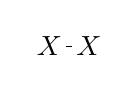
\begin{tikzpicture}[baseline={([yshift=-.5ex]current bounding box.center)}]
	\path (0,0) node (A) {$X$} ++ (0.5,0) node (B) {$X$};
	\draw (A) -- (B);
\end{tikzpicture}
\end{align}

We choose a particular 1-element set $\{*\}$ that acts as the identity in the sense that $\{*\}\times A\cong A\times \{*\} \cong A$ for any set $A$. The erase map $\text{del}_X:X\kto \{*\}$ defined by $(\text{del}_X)(*|x) = 1$ is a Markov kernel that ``discards the input''. It is drawn as a fuse:

\begin{align}
	\text{del}_X&:=\begin{tikzpicture}[baseline={([yshift=-.5ex]current bounding box.center)}]
	\path (0,0) ++ (1,0) node (B) {$X$};
	\draw[-{Rays[n=8]}] (A) -- (B);
\end{tikzpicture}
\end{align}

The copy map $\text{copy}_X:X\kto X\times X$ defined by $(\text{copy}_X)(x',x''|x)=\llbracket x=x' \rrbracket \llbracket x=x'' \rrbracket$ is a Markov kernel that makes two identical copies of the input. It is drawn as a fork:

\begin{align}
	\text{copy}_X&:=\begin{tikzpicture}[baseline={([yshift=-.5ex]current bounding box.center)}]
	\path (0,0) node (A) {$X$} 
	++ (0.5,0) node[copymap] (copy0) {}
	++ (0.5,0.15) node (B) {$X$}
	+ (0,-0.3) node (C) {$X$};
	\draw (A) -- (copy0) to [out=45,in=180] (B) (copy0) to [out=-45, in=180] (C);
\end{tikzpicture}
\end{align}

The swap map $\text{swap}_{X,Y}:X\times Y\kto Y\times X$ defined by $(\text{swap}_{X,Y})(y',x'|x,y)=\llbracket x=x' \rrbracket\llbracket y=y' \rrbracket$ swaps two inputs, and is represented by crossing wires:

\begin{align}
	\text{swap}_X &:=  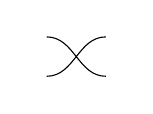
\begin{tikzpicture}[baseline={([yshift=-.5ex]current bounding box.center)}]
		\path (0,0) node (A) {} 
		+ (0,-0.5) node (B) {}
		++ (1,0) node (C) {}
		+ (0,-0.5) node (D) {};
		\draw (A) to [out=0,in=180] (D) (B) to [out=0, in=180] (C);
	\end{tikzpicture}
\end{align}

Because we anticipate that the graphical notation will be unfamiliar to many, we will also include translations to more familiar notation.

\subsection{Combs: Markov kernels with gaps in them}

Consider the Markov kernels $\kernel{K}:W\kto Y$, $\kernel{L}:Y\times X\kto Z$ and $\kernel{M}:W\times X\kto Y\times Z$ defined as

\begin{align}
	\kernel{M} = \tikzfig{2_comb}\label{eq:2comb_M}
\end{align}

Following the rules above, we can translate this to ordinary notation by first breaking it down into products and tensor products, and then evaluating these products

\begin{align}
	\kernel{M}(y,z|w,x) &= (\kernel{K}\otimes \text{id}_X)[(\text{copy}_Y\otimes \text{id}_X)(\text{id}_Y\otimes\kernel{L})](y,z|w,x)\\
						&= \sum_{x'\in X,y'\in Y} \kernel{K} (y'|w) \llbracket x=x' \rrbracket [(\text{copy}_Y\otimes \text{id}_X)
						(\text{id}_Y\otimes\kernel{L})](y,z|y',x')\\
						&= \sum_{y'\in Y}  \kernel{K} (y'|w)[(\text{copy}_Y\otimes \text{id}_X)
						(\text{id}_Y\otimes\kernel{L})](y,z|y',x)\\
						&= \sum_{y'}  \kernel{K} (y'|w) \sum_{x'\in X,y'',y'''\in Y}\llbracket y'=y''\rrbracket\llbracket y'=y''' \rrbracket \llbracket x = x' \rrbracket \llbracket y''=y \rrbracket \kernel{L} (z|y''',x') (y,z|y',x')\\
						&= \kernel{K}(y|w)\kernel{L}(z|y,x)
\end{align}

Now, if we are given additionally $\kernel{J}:Y\kto X$, we can define a new Markov kernel $\kernel{N}:W\kto Z$:

\begin{align}
	\kernel{N} = \tikzfig{2comb_inserted}\label{eq:2comb_winsert}
\end{align}

For the following translation, we will apply the following shorthands: for arbitrary $\kernel{A}:X\times Y\to Z$, $\kernel{B}:W\to Y$

\begin{align}
 (\text{Id}_X\otimes \kernel{W})\kernel{A}(z|x,w) &= \sum_{y'\in Y, x'\in X}\llbracket x=x' \rrbracket \kernel{W}(y'|w) \kernel{B}(z|x',y')\\
										   &= \sum_{y'\in Y} \kernel{W}(y'|w) \kernel{B}(z|x,y')
\end{align}

That is, an identity map passes along its input to the next kernel in the product. In addition, for arbitrary $\kernel{B}: X\times Y\times Y\to Z$ (where we apply the above shorthand immediately):

\begin{align}
 (\text{Id}_X\otimes \text{copy}_Y)\kernel{B}(z|x,y) &= \sum_{y',y''\in Y}\text{copy}_Y(y',y''|y)\kernel{B}(z|x,y',y'')\\
										   &= \kernel{B}(z|x,y,y)
\end{align}

That is, the copy map passes along two copies of its input to the next kernel in the product. Finally, for $\kernel{C}^n:Y^n\to Z$, define $(y)^{n}=(y|i\in[n])$:

\begin{align}
	\text{copy}^n_Y &:= \begin{cases}
	\text{copy}^{n-1}_Y(\text{Id}_{Y^{n-2}}\otimes \text{copy}_Y) & n>2\\
	\text{copy}_Y & n=2
	\end{cases}\\
	(\text{copy}^2_Y\kernel{C}^2)(z|y) &= \kernel{C}^2(z|y,y)\\
	\text{ suppose for induction } (\text{copy}^{n-1}_Y\kernel{C}^{n-1})(z|y) &= \kernel{C}^{n-1}(z|(y)^{n-1})\\
	\text{ then }(\text{copy}^n_Y\kernel{C}^n)(z|y) &= (\text{copy}^{n-1}_Y(\text{Id}_{Y^{n-2}}\otimes \text{copy}_Y)\kernel{C}^n)(z|y)\\
									 &= \sum_{y'\in Y^{n-1}}(\text{Id}_{Y^{n-2}}\otimes \text{copy}_Y)(\mathbf{y}'|(y)^{n-1})\kernel{C}^n(z|\mathbf{y}')\\
									 &= \kernel{C}^n(z|(y)^n)
\end{align}

Using these shorthands, we can translate Equation \ref{eq:2comb_winsert} to

\begin{align}
	\kernel{N}(z,x,y|w) &= [\kernel{K}\text{copy}^3_Y(\text{Id}_Y\otimes\kernel{J}\otimes \text{Id}_Y)(\text{Id}_Y \otimes \text{copy}_X\otimes \text{Id}_Y)(\kernel{L}\otimes \text{Id}_X\otimes \text{Id}_Y)] (z,x,y|w)\\
					&= \sum_{y'\in Y} \kernel{K}(y'|w)  [(\text{Id}_Y\otimes\kernel{J}\otimes \text{Id}_Y)(\text{Id}_Y\otimes\text{copy}_X\otimes \text{Id}_Y)(\kernel{L}\otimes \text{Id}_X\otimes \text{Id}_Y)] (z,x,y|y',y',y')\\
					&= \sum_{y'\in Y,x'\in X} \kernel{K}(y'|w)\kernel{J}(x'|y')[\kernel{L}\otimes \text{Id}_X\otimes \text{Id}_Y] (z,x,y|y',x',x',y')\\
					&= \kernel{K}(y|w) \kernel{J}(x|y) \kernel{L}(z|y,x)\\
\end{align}

We say $\kernel{M}$ is a \emph{2-comb} after \citet{chiribella_quantum_2008}. Similar to the copy-product we defined between two appropriately typed Markov kernels, we can define an insert-product between a 2-comb and an appropriately defined insert.

Specifically, given a 2-comb $\kernel{M}$ defined as in Equation \ref{eq:2comb_M} and a Markov kernel $\kernel{J}:Y\kto X$, we define $\text{Insert}(\kernel{M},\kernel{J})$ to be the right hand side of Equation \ref{eq:2comb_winsert}. We can depict this informally as follows:

\begin{align}
	\text{Insert}\left(\tikzfig{insert_opn2}\right) &= \tikzfig{2comb_inserted}\label{eq:insert_op}
\end{align}

The insert-product places $\kernel{J}$ in the matching slot in $\kernel{M}$, and also copies both the input and output of $\kernel{J}$ to the output of the result. Just as copy-products extend conditional probabilities, insert-products extend probability combs.

Note that if $W=Y=\{*\}$, then $\text{Insert}(\kernel{M},\kernel{J})\cong \kernel{J}\odot \kernel{M}$.

\subsection{Probability combs}

We will use probability 2-combs to define probability models with ``conditional probability shaped gaps''. Just as in Section \ref{sec:validity_of_gapprob}, our main concern is whether a probability 2-comb is \emph{validly extendable}.

\begin{definition}[Probability 2-comb]
Given $\RV{W}:\Omega\to W$, $\RV{X}:\Omega\to X$, $\RV{Y}:\Omega\to Y$, $\RV{Z}:\Omega\to Z$, a probability 2-comb $\prob{P}^{\RV{X}|\RV{W}\square\RV{Z}|\RV{Y}}:Y\kto X\times Z$ is a Markov kernel with components $\prob{P}^{\RV{X}|\RV{W}}$ and $\prob{P}^{\RV{Z}|\RV{WXY}}$ defined by
\begin{align}
	\prob{P}^{\RV{X}|\RV{W}\square\RV{Z}|\RV{Y}} &= \tikzfig{probability_2_comb}
\end{align}
\end{definition}

Inserting a conditional probability into a probability 2-comb yields a condiitonal probability.

\begin{definition}[Valid probability 2-comb]
Given $(\Omega,\sigalg{F})$, $\RV{W}:\Omega\to W$, $\RV{X}:\Omega\to X$, $\RV{Y}:\Omega\to Y$ and $\RV{Z}:\Omega\to Z$ a \emph{valid probability 2-comb} $\prob{P}^{\RV{X}|\RV{W}\square\RV{Z}|\RV{Y}}$ is a Markov kernel $Y\kto X\times Z$ such that:
\begin{align}
	\forall w\in W, A\in \sigalg{X}, y\in Y,C\in\sigalg{Z}: &\RV{W}^{-1}(w)\cap\RV{X}^{-1}(A)\cap \RV{Y}^{-1}(y)\cap \RV{Z}^{-1}(C) = \emptyset\\ 
	\implies &\left(\prob{P}^{\RV{X}|\RV{W}\square\RV{Z}|\RV{Y}}(A\times C|w,y) = 0\right) \lor \\
	&\left(\RV{W}^{-1}(w)\cap\RV{X}^{-1}(A)\cap\RV{Y}^{-1}(y) = \emptyset\right)
\end{align}
\end{definition}

Calid conditional probabilities were precisely those that, given any valid probability distribution, could be extended to valid probability distributions. Analogously, valid probability 2-combs are precisely those that, given any valid conditional probability, can be extended to valid conditional probabilities.

\begin{theorem}[Extension of valid probability 2-combs]
Given $(\Omega,\sigalg{F})$, $\RV{W}:\Omega\to W$, $\RV{X}:\Omega\to X$, $\RV{Y}:\Omega\to Y$ and $\RV{Z}:\Omega\to Z$, a probability 2-comb $\prob{P}^{\RV{X}|\RV{W}\square\RV{Z}|\RV{Y}}$ is valid if and only if for any valid conditional probability $\prob{P}^{\RV{Z}|\RV{X}}$, $\text{insert}(\prob{P}^{\RV{X}|\RV{W}\square\RV{Z}|\RV{Y}},\prob{P}^{\RV{Z}|\RV{X}})$ is a valid conditional probability.
\end{theorem}

\begin{proof}

\end{proof}

It appears that we may be able to extend this theory to $n$-combs, where valid $n$-combs are those that can have $n-1$-combs inserted to yield valid $n-1$-combs. We don't develop that theory here, though.

\subsection{What goes wrong with truncated factorisation?}

A \emph{model} is a collection of conditional probabilities. For example, we could have $\{\prob{P}^{\RV{X}|*},\prob{P}^{\RV{Y}|\RV{X}}\}$. We use the convention that conditional probabilities with the same base letter all belong to the same model. Whether a particular model is ``correct'' is a difficult question to answer, and indeed a difficult question to pose. However, we can specify some necessary conditions that must hold. Informally, these are:

\begin{enumerate}
	\item All conditional probabilities assign probability 0 to contradictions and probability 1 to tautologies
	\item There exists a $\RV{Y}:\Omega\to Y$ and a master probability $\prob{P}^{\RV{I}|\RV{Y}}$ compatible with all the conditional probabilities in the model
\end{enumerate}

The first condition is not standard, while the second condition is.

\begin{definition}[Probability 0 to contradictions]\label{def:prob_0_contradiction}
A conditional probability $\prob{P}^{\RV{Y}|\RV{X}}$ assigns probability 0 to contradictions if 
\begin{align}
	(\RV{X}^{-1}(x)\neq \emptyset)\land (\RV{X}^{-1}(x)\cap \RV{Y}^{-1}(A) = \emptyset) \implies\prob{P}^{\RV{Y}|\RV{X}}(A|x) = 0
\end{align}
\end{definition}

This condition says: if, according to my chosen variables, $\RV{X}$ may potentially yield $x$ but $\RV{Y}$ cannot possibly yield $A$ when $\RV{X}$ yields $x$, then the conditional probability must assign a probability of 0 to $\RV{Y}$ yielding $A$ given $\RV{X}$ yields $x$. This is non-standard, because the condition is not that the \emph{probability} that $\prob{P}^\RV{X}(x)$ is nonzero (a quantity which may not be defined), but simply that $x$ is in the range of the variable $\RV{X}$. This is required if $\prob{P}^{\RV{X}}$ is not defined. \citet{hajek_what_2003} argues that it is desirable even if $\prob{P}^{\RV{X}}$ is defined, though in that case it would normally have no impact on questions of interest. See also \citet{renyi_conditional_1956}.

It is a consequence of Definition \ref{def:prob_0_contradiction} that $\prob{P}^{\RV{Y}|\RV{X}}$ assigns probability 1 to tautologies. If $\RV{X}\bowtie x\subset \RV{Y}\bowtie A$ then $\RV{X}^{-1}(x)\cap \RV{Y}^{-1}(A^C) = \emptyset$, and hence $\prob{P}^{\RV{Y}|\RV{X}}(A^C|x) = 0$ so $\prob{P}^{\RV{Y}|\RV{X}}(A|x) = 1$.

\begin{definition}[Compatible master condtional probability]\label{def:compat_master}
We say a conditional probability $\prob{P}^{\RV{X}_i|\RV{X}_j}$ is compatible with $\prob{P}^{\RV{I}|\RV{Y}}$ if
\begin{align}
	\prob{P}^{\RV{I}|\RV{Y}}((\RV{X}_i,\RV{X}_j)\bowtie A\times B|c) &= \int_A \prob{P}^{\RV{X}_{i}|\RV{X}_j}(B|\RV{X}_j(\omega))\prob{P}^{\RV{I}|\RV{Y}}(d\omega|c) &\forall c\in Y:\prob{P}^{\RV{I}|\RV{Y}}(\RV{X}_j\bowtie A|c)>0 \label{eq:ssc_2}
\end{align}
\end{definition}

There is one final difference between our approach and the standard one: we say a model is a collection of conditional probabilities compatible with some $\prob{P}^{\RV{I}|\RV{Y}}$, while the standard approach is to say that $\prob{P}^{\RV{I}|\RV{Y}}$ is the model and goes on to define how the conditional probabilities can be derived from it. The difference here is that \textbf{our approach implies that conditional probabilities in a model are unique}. If there are multiple Markov kernels that satisfy Equation \ref{eq:ssc_2}, we assume that one of these is chosen somehow. 


\subsection{Composition and probability with variables}

We then need a notion of Markov kernels that ``maps between variables''. An \emph{indexed Markov kernel} is such a thing.

\begin{definition}[Indexed Markov kernel]
Given variables $\RV{X}:\Omega\to A$ and $\RV{Y}:\Omega\to B$, an indexed Markov kernel $\kernel{K}:\RV{X}\kto \RV{Y}$ is a triple $(\kernel{K}',\RV{X},\RV{Y})$ where $\kernel{K}':A\kto B$ is the \emph{underlying kernel}, $\RV{X}$ is the \emph{input index} and $\RV{Y}$ is the \emph{output index}.
\end{definition}

For example, if $\kernel{K}:(\RV{A}_1,\RV{A}_2)\to \Delta(\RV{B}_1,\RV{B}_2)$, for example, we can draw:

\begin{align}
	\kernel{K} := \begin{tikzpicture}[baseline={([yshift=-.5ex]current bounding box.center)}]
	\path (0,0) node (A1) {$\RV{A}_1$}
	+ (0,-0.3) node (A2) {$\RV{A}_2$}
	++ (0.7,-0.15) node[kernel] (K) {$\kernel{K}$}
	++ (0.7,0.15) node (B1) {$\RV{B}_1$}
	+ (0,-0.3) node (B2) {$\RV{B}_2$};
	\draw (A1) -- ($(K.west) + (0,0.15)$) (A2) -- ($(K.west) + (0,-0.15)$);
	\draw (B1) -- ($(K.east) + (0,0.15)$) (B2) -- ($(K.east) + (0,-0.15)$);
\end{tikzpicture}
\end{align}

or

\begin{align}
	\kernel{K} = \begin{tikzpicture}[baseline={([yshift=-.5ex]current bounding box.center)}]
	\path (0,0) node (A1) {$(\RV{A}_1,\RV{A}_2)$}
	++ (1.3,0) node[kernel] (K) {$\kernel{K}[\model{L}]$}
	++ (1.3,0.) node (B1) {$(\RV{B}_1,\RV{B}_2)$};
	\draw (A1) -- (K) -- (B1);
\end{tikzpicture}
\end{align}

We define the product of indexed Markov kenrnels $\kernel{K}:\RV{X}\kto \RV{Y}$ and $\kernel{L}:\RV{Y}\kto \RV{Z}$ as the triple $\kernel{K}\kernel{L}:=(\kernel{K}'\kernel{L}',\RV{X},\RV{Z})$.

Similarly, the tensor product of $\kernel{K}:\RV{X}\kto\RV{Y}$ and $\kernel{L}:\RV{W}\kto\RV{Z}$ is the triple $\kernel{K}\otimes\kernel{L}:=(\kernel{K}'\otimes\kernel{L}',(\RV{X},\RV{W}),(\RV{Y},\RV{Z}))$.

We define $\text{Id}_{\RV{X}}$ to be the model $(\text{Id}_X,\RV{X},\RV{X})$, and similarly the indexed versions $\text{del}_{\RV{X}}$, $\text{copy}_{\RV{X}}$ and $\text{swap}_{\RV{X},\RV{Y}}$ are obtained by taking the unindexed versions of these maps and attaching the appropriate random variables as indices. Diagrams are the diagrams associated with the underlying kernel, with input and output wires annotated with input and output indices.

The category of indexed Markov kernels as morphisms and variables as objects is a Markov category (Appendix \ref{sec:app_mcat}), and so a valid derivation based on the string diagram language for Markov categories corresponds to a valid theorem in this category. However, most of the diagrams we can form are not viable candidates for models of our variables. For example, if $\RV{X}$ takes values in $\{0,1\}$ we can propose an indexed Markov kernel $\kernel{K}:\RV{X}\kto\RV{X}$ with $\kernel{K}_a^{\prime b}=0.5$ for all $a, b$. However, this is not a useful model of the variable $\RV{X}$ -- it expresses something like ``if we know the value of $\RV{X}$, then we belive that $\RV{X}$ could take any value with equal probability''.

We define a \emph{model} as ``an indexed Markov kernel that assigns probability 0 to things known to be contradictions''. A contradiction is a simultaneous assignment of values to the variables $\RV{X}$ and $\RV{Y}$ such that there is no value of $\omega$ under which they jointly take these values. Unless the value assignment to the domain variable is itself contradictory, we hold that any valid model must assign probability zero to such occurrences.

\begin{definition}[Probabilistic model]
An indexed Markov kernel $(\kernel{K}',\RV{X},\RV{Y})$ is a \emph{probabilistic model} (``model'' for short) if it is \emph{consistent}, which means it assigns probability 0 to contradictions:
\begin{align}
	f_{\RV{X}}^{-1}(a)\cap f_{\RV{Y}}^{-1}(b) = \emptyset \implies \left(\kernel{K}_{a}^{\prime b} = 0\right) \lor \left(f_{\RV{X}}^{-1}(a) = \emptyset\right)
\end{align}
A \emph{probability model} is a model where the underlying kernel $\kernel{K}'$ has the unit $\RV{I}$ as the domain. We use the font $\model{K}$ to distinguish models from arbitrary indexed Markov kernels.
\end{definition}

Consistency implies that for any $\model{K}:\RV{X}\kto\RV{Y}$, if $f_{\RV{Y}}=g\circ f_{\RV{X}}$ then $\model{K}_x^{g(x)}=1$. A particularly simple case of this is a model $\model{L}:\RV{X}\kto\RV{X}$, which must be such that $\model{L}_x^x=1$. \citet{hajek_what_2003} has pointed out that standard definitions of conditional probability allow the conditional probability to be arbitrary on a set of measure zero, even though ``the probability $\RV{X}=x$, given $\RV{X}=x$'' should obviously be 1.

We take the idea of marginal distributions as fundamental.

\begin{definition}[Marginal distribution]
Given a model $\model{K}:\RV{X}\kto(\RV{Y},\RV{Z})$, the marginal distribution of $\RV{Y}$, written $\model{K}^{\RV{Y}|\RV{X}}$, is obtained by marginalising over $\RV{Z}$:
\begin{align}
	\model{K}^{\RV{Y}|\RV{X}} &:= \tikzfig{marginal}\\
	&\iff\\
	(\model{K}^{\RV{Y}|\RV{X}})_x^y &= \sum_{z\in Z} \kernel{K}_x^{\prime yz}
\end{align}
\end{definition}

\begin{definition}[Disintegration]
Given a model $\model{K}:\RV{X}\kto(\RV{Y},\RV{Z})$, a disintegration $\model{L}:(\RV{X},\RV{Y})\kto \RV{Z}$ $\RV{Y}$, written $\model{K}^{\RV{Y}|\RV{X}}$, is obtained by marginalising over $\RV{Z}$
\end{definition}

We can always get a valid model by adding a copy map to a valid model, and conversely all valid models with repeated codomain variables must contain copy maps.

\begin{lemma}[Output copies of the same variable are identical]\label{lem:nocopy1}
For any $\kernel{K}:\RV{X}\kto (\RV{Y},\RV{Y},\RV{Z})$, $\kernel{K}$ is a model iff there exists some $\model{L}:\RV{X}\kto (\RV{Y},\RV{Z})$ such that
\begin{align}
		\kernel{K} &= \tikzfig{compose_with_copymap}\\
		&\iff \\
		\kernel{K}_{x}^{\prime y,y',z} &= \llbracket y=y' \rrbracket\kernel{L}_{x}^{\prime y,z}\\
\end{align}
\end{lemma}


\begin{proof}
$\implies$
For any $\omega,x,y,y',z$:
\begin{align}
	(\RV{X},\RV{Y},\RV{Y},\RV{Z})_\omega^{x,y,y',z} &= \llbracket f_{\RV{Y}}(\omega)=y \rrbracket \llbracket f_{\RV{Y}}(\omega)=y' \rrbracket (\RV{X},\RV{Z})_\omega^{x,z} \\
	&= \llbracket y=y' \rrbracket \llbracket f_{\RV{Y}}(\omega)=y \rrbracket(\RV{X},\RV{Z})_\omega^{x,z}
\end{align}
Therefore, by consistency, for any $x,y,y',z$, $y\neq y'\implies \kernel{K}_{x}^{\prime yy'z}=0$. Define $\kernel{L}$ by $\kernel{L}_x^{\prime y, z} := \kernel{K}_x^{\prime y y z}$. The fact that $\model{L}$ is a model follows from the assumption that $\model{K}$ is. Then
\begin{align}
	\kernel{K}_{x}^{\prime y,y',z} &= \llbracket y=y' \rrbracket\kernel{L}_{x}^{\prime y,z}
\end{align}
$\Leftarrow$
If $\model{L}$ is a model, then for any $x,x',y,z$, 
\begin{align}
\llbracket y=y'\rrbracket \model{L}_{x}^{\prime y,z}>0&\implies y=y'\land \model{L}_{x}^{\prime y,z}>0\\
													  &\implies \left(f_{\RV{X}}^{-1}(x)=\emptyset \right)\lor \left(f_{\RV{X}}^{-1}(x)\cap f_{\RV{Y}}^{-1}(y) \cap f_{\RV{Y}}^{-1}(y)\cap f_{\RV{Z}}^{-1}(z)\neq\emptyset \right)\\
\end{align}
\end{proof}

We can always get a valid model by copying the input to the output of a valid model, and conversely all valid models where there is a variable shared between the input and the output must copy that input to the output.

\begin{lemma}[Copies shared between input and output are identical]\label{lem:nocopy2}
For any $\kernel{K}:(\RV{X},\RV{Y})\kto (\RV{X},\RV{Z})$, $\kernel{K}$ is a model iff there exists some $\model{L}:(\RV{X},\RV{Y})\kto \RV{Z}$ such that
\begin{align}
	 \kernel{K} &= \tikzfig{precompose_with_copymap}\\
	 &\iff\\
	 \kernel{K}_{x,y}^{\prime x',z} &= \llbracket x=x'\rrbracket \kernel{L}_{\prime x,y}^{z}
\end{align}
\end{lemma}

\begin{proof}
$\implies$
For any $\omega,x,y,y',z$:
\begin{align}
	(\RV{X},\RV{Y},\RV{Y},\RV{Z})_\omega^{x,y,y',z} &= \llbracket f_{\RV{Y}}(\omega)=y \rrbracket \llbracket f_{\RV{Y}}(\omega)=y' \rrbracket (\RV{X},\RV{Z})_\omega^{x,z} \\
	&= \llbracket y=y' \rrbracket \llbracket f_{\RV{Y}}(\omega)=y \rrbracket(\RV{X},\RV{Z})_\omega^{x,z}
\end{align}
Therefore, by consistency, for any $x,y,y',z$, $x\neq x'\implies \model{K}_{x,y}^{\prime x'z}=0$. Define $\kernel{L}$ by $\kernel{L}_{x,y}^{\prime x', z} := \model{K}_{x,y}^{\prime x, y}$. The fact that $\kernel{L}$ is a model follows from the assumption that $\model{K}$ is a model. Then
\begin{align}
	\kernel{K}_{x, y}^{\prime x', z} &= \llbracket x=x' \rrbracket\kernel{L}_{x,y}^{\prime z}
\end{align}
$\Leftarrow$
If $\model{L}$ is a model, then for any $x,x',y,z$, 
\begin{align}
\llbracket x=x'\rrbracket \model{L}_{ x,y}^{\prime z}>0&\implies x=x'\land \model{L}_{ x,y}^{\prime z}>0\\
													  &\implies \left( f_{\RV{X}}^{-1}(x)\cap f_{\RV{Y}}^{-1}(y)=\emptyset \right)\lor \left(f_{\RV{X}}^{-1}(x)\cap f_{\RV{X}}^{-1}(x)\cap f_{\RV{Y}}^{-1}(y)\cap f_{\RV{Z}}^{-1}(z)\neq\emptyset \right)\\
\end{align}
\end{proof}

Consistency along with the notion of marginal distributions implies that, given some $\RV{X}$ and some $\model{K}:\RV{Y}\kto\text{Id}_\Omega$, the pushforward $\model{K}\model{X}$ is the unique model $\RV{Y}\kto \RV{X}$ that can be paired (Definition \ref{def:pairing}) with $\model{K}$. This is shown in Lemma \ref{lem:pushforward}.

\begin{lemma}[Uniqueness of models with the sample space as a domain]\label{lem:uniq_model}
For any $\RV{X}:\Omega\to A$, there is a unique model $\model{X}:\text{Id}_\Omega\kto \RV{X}$ given by $\model{X}:=(\RV{X},\text{Id}_\Omega,\RV{X})$.
\end{lemma}

\begin{proof}
$\RV{X}$ is a Markov kernel mapping from $\Omega\to A$, so it is a valid underlying kernel for $\model{X}$, and $\model{X}$ has input and output indices matching its signature. We need to show it satisfies consistency.

For any $\omega\in \Omega$, $a\in A$
\begin{align}
	\max_{\omega\in \Omega}(\text{Id}_\Omega,\RV{X})_{\omega}^{\omega',a} &= \max_{\omega\in \Omega} \llbracket \omega = \omega' \rrbracket \llbracket \omega = f_{\RV{X}}(a) \rrbracket\\
	&= \llbracket \omega = f_{\RV{X}}(a) \rrbracket\\
	&= \kernel{X}_\omega^a
\end{align}
Thus $\model{X}$ satisfies consistency.

Suppose there were some $\model{K}:\text{Id}_\Omega\kto \RV{X}$ not equal to $\RV{X}$. Then there must be some $\omega\in \Omega$, $b\in A$ such that $\model{K}_\omega^b\neq 0$ and $f_{\RV{X}}(\omega)\neq b$. Then
\begin{align}
	\max_{\omega\in \Omega}(\text{Id}_\Omega,\RV{X})_{\omega}^{\omega',a} &= \max_{\omega\in \Omega} \llbracket \omega = \omega' \rrbracket \llbracket \omega = f_{\RV{X}}(b) \rrbracket\\
	&= \llbracket \omega = f_{\RV{X}}(b) \rrbracket\\
	&= 0\\
	&< \model{K}_\omega^b
\end{align}
Thus $\model{K}$ doesn't satisfy consistency.
\end{proof}

% \begin{corollary}[Uniqueness of joint models]\label{cor:uniq_joint}
% For any $\RV{X}:\Omega\to A$, there is a unique model $\model{X}:\text{Id}_\Omega\kto (\RV{X},\text{Id}_{\Omega})$.
% \end{corollary}

% \begin{proof}
% Apply Lemma \ref{lem:nocopy2} to the model $\model{X}$ from Lemma \ref{lem:uniq_model}.
% \end{proof}

\begin{definition}[Pairing]\label{def:pairing}
Two models $\model{K}:\RV{X}\kto \RV{Y}$ and $\model{L}:\RV{X}\kto \RV{Z}$ can be \emph{paired} if there is some $\model{M}:\RV{X}\kto (\RV{Y},\RV{Z})$ such that $\model{K}=\model{M}^{\RV{Y}|\RV{X}}$ and $\model{L}=\model{M}^{\RV{Z}|\RV{X}}$.
\end{definition}

\begin{lemma}[Pushforward model]\label{lem:pushforward}
Given any model $\model{K}:\RV{Y}\kto \text{Id}_\Omega$ and any $\RV{X}$, there is a unique $\model{L}:\RV{Y}\kto \RV{X}$ that can be paired with $\model{K}$, and it is given by $(\kernel{L}^a_b = \sum_{\omega\in f_{\RV{X}}^{-1}(a)} \kernel{K}_b^{\omega}$.
\end{lemma}

\begin{proof}
Suppose that there is some $\model{L}$ that can be paired with $\model{K}$ via some $\model{M}:\RV{Y}\kto(\text{Id}_\Omega,\RV{X})$. Then, by the existence of disintegrations, there must be some $\model{N}:\text{Id}_{\Omega}\kto \RV{X}$ such that
\begin{align}
	\model{M}&=\tikzfig{disintegration_omega}
\end{align}
By Corollary \ref{cor:uniq_joint}, there is only one model $\model{N}:\text{Id}_{\Omega}\kto \RV{X}$ is unique and equal to $\model{X}:=(\RV{X},\text{Id}_\Omega,\RV{X})$.

It remains to be shown that $\model{M}$ is also a model. We already know that $\model{K}$ is consistent with respect to $(\RV{Y},\text{Id}_\Omega)$ and $\model{L}$ is consistent with respect to $(\text{Id}_\Omega,\RV{X})$. $\model{M}$ must be consistent with respect to $(\RV{Y},\text{Id}_\Omega,\RV{X})$. Consider any $x\in X$, $\omega\in \Omega$, $y\in Y$ such that $f_{\RV{X}}^{-1}(x)\cap \{\omega\}\neq \emptyset$ and $f_{\RV{Y}}^{-1}(y)\cap\{\omega\}\neq \emptyset$. Trouble might arise if $f_{\RV{X}}^{-1}(x)\cap \{\omega\} \cap f_{\RV{Y}}^{-1}(y)=\emptyset$, but this is obviously impossible as $\omega\in f_{\RV{X}}^{-1}(x)$ and $\omega\in f_{\RV{Y}}^{-1}(y)$.

Finally, for any $a\in A$, $b\in B$
\begin{align}
	(\model{K}\model{X})^a_b &= \sum_{\omega\in \Omega} \model{P}_b^\omega\RV{X}_\omega^a\\
						 &= \sum_{\omega\in \Omega} \model{P}_b^\omega \llbracket a = f_{\RV{X}}(\omega) \rrbracket\\
						 &= \sum_{\omega\in f^{-1}(a)} \model{P}_b^{\omega}
\end{align}
\end{proof}

\begin{corollary}[Pushforward probability model]\label{corr:pushforward}
Given any probability model $\model{P}:\RV{I}\kto \text{Id}_\Omega$, there is a unique model $\model{P}^{\RV{X}}:\RV{I}\kto \RV{X}$ such that $\model{P}^{\RV{X}}=\model{P}\model{Q}$ for some $\model{Q}:\text{Id}_\Omega\to \RV{X}$, and it is given by $(\model{P}^{\RV{X}})^a_b = \sum_{\omega\in f^{-1}(a)} \model{P}_b^{\omega}$.
\end{corollary}

\begin{proof}
Apply Lemma \ref{lem:pushforward} to a model $\model{P}:\RV{I}\kto\text{Id}_{\Omega}$.
\end{proof}

The following lemmas can help us check whether an indexed Markov kernel is a valid model.



We take the following term from \citet{constantinou_extended_2017}. Our definition is equivalent to unconditional variation independence in that paper.

\begin{definition}[Variation independence]
Two variables $\RV{X}:\Omega\kto X$ and $\RV{Y}:\Omega\kto Y$ are variation independent, written $\RV{X}\perp_v \RV{Y}$, if for all $y\in f_\RV{Y}(\Omega)R(f_{\RV{Y}})$
\begin{align}
 f_\RV{Y}(\Omega) \times f_{\RV{X}}(\Omega) = \{(f_{\RV{Y}}(\omega),f_{\RV{X}}(\omega))|\omega\in \Omega\}
\end{align}
\end{definition}

If a collection of variables is variation independent and surjective, then an arbitrary indexed Markov kernel labelled with these variables is a model.

\begin{lemma}[Consistency via variation conditional independence]\label{lem:var_indep}
Given an indexed Markov kernel $\kernel{K}:\RV{X} \kto \RV{Y}$ with $\RV{X}:\Omega\kto X$ and $\RV{Y}:\Omega\kto Y$, if $f_\RV{Y}$ is surjective and $\RV{Y}\perp_v \RV{X}$ then $\kernel{K}$ is a model.
\end{lemma}

\begin{proof}
By variation independence and surjectivity of $f_{\RV{Y}}$, for any $x\in X$, $y\in Y$, $f_{\RV{X}}^{-1}(x)\cap f_{\RV{Y}}^{-1}(y) = \emptyset \implies f_{\RV{X}}^{-1}(x) = \emptyset$. Thus the criterion of consistency places no restrictions on $\kernel{K}$.
\end{proof}

\todo[inline]{I think Lemmas \ref{lem:nocopy1} and \ref{lem:nocopy2} might be sufficient to offer diagrammatic checks of consistency if all variables that are not identical are variation independent. This is probably an interesting result, but I'm not sure if it's a higher priority than filling out the rest of the content.}

Alternatively, if we have a strictly positive indexed Markov kernel that is known to be a model, we can conclude that arbitrary indexed Markov kernels with appropriate labels are also models.

\begin{lemma}[Consistency via positive models]\label{lem:avoid_contradic}
Given a model $\model{K}:\RV{X}\kto (\RV{Y},\RV{Z})$, if an indexed Markov kernel $\kernel{L}:(\RV{X},\RV{Y})\kto \RV{Z}$ has the property $\kernel{K}_x^{\prime yz}=0\implies \kernel{L}_{xy}^{\prime z}=0$ then $\kernel{L}$ is also a model.
\end{lemma}

\begin{proof}
Because $\model{K}$ is a model,
\begin{align}
	\kernel{L}_{xy}^{\prime z}>0 &\implies \kernel{K}_x^{\prime yz} >0 \\
	&\implies \left( f_\RV{X}^{-1}(x)\cap f_\RV{Y}^{-1}(y)\cap f_\RV{Z}^{-1}(z) \neq \emptyset \right) \lor \left(f_\RV{X}^{-1}(x) = \emptyset \right)\\
	&\implies \left( f_\RV{X}^{-1}(x)\cap f_\RV{Y}^{-1}(y)\cap f_\RV{Z}^{-1}(z) \neq \emptyset \right) \lor \left(f_\RV{X}^{-1}(x)\cap f_{\RV{Y}}^{-1}(y) = \emptyset \right)
\end{align}
\end{proof}

\subsection{Truncated factorisation with variables}

At this point, we can represent Equation \ref{eq:truncated_fac} using models. Suppose $P^{\RV{Y|XZ}}$ is an model $\model{K}:(\RV{X}, \RV{Z})\kto \RV{Y}$ and $\prob{P}^{\RV{Z}}$ an model $\model{L}:\{*\}\kto \RV{Z}$. Then we can define an indexed Markov kernel $\kernel{M}:\RV{X}\kto \RV{X}, \RV{Z}$ representing $x\mapsto \prob{P}^{\RV{YZ}}_{x}(y,z)$ by

\begin{align}
	\kernel{M}&:= \tikzfig{truncated_factorisation_labeled}\label{eq:tfac_labeled}
\end{align}

Equation \ref{eq:tfac_labeled} is almost identical to Equation \ref{eq:tfac_setted}, except it now specifies which variables each measure applies to, not just which sets they take values in. Like the original Equation \ref{eq:truncated_fac}, there is no guarantee that $\kernel{M}$ is actually a model. If $f_\RV{X}=g\circ f_\RV{Z}$ for some $g:Z\to X$ and $X$ has more than 1 element, then the rule of consistency will rule out the existence of any such model.

If we want to use $\kernel{M}$, we want it at minimum to satisfy the consistency condition. One approach we could use is to check the result using Lemmas \ref{lem:nocopy1} to \ref{lem:avoid_contradic}, although note that \ref{lem:var_indep} and \ref{lem:avoid_contradic} are sufficient conditions, not necessary ones.

\subsection{Sample space models and submodels}

Instead of trying to assemble probability models as in Equation \ref{eq:tfac_labeled}, we might try to build probability models in a manner closer to the standard setup -- that is, we start with a sample space model (or a collection of sample space models) and work with marginal and conditional probabilities derived from these, without using any non-standard model assemblies.

A sample space model is any model $\kernel{K}:\RV{X}\kto \text{Id}_\Omega$. We expect that the collection of models under consideration will usually be defined on some small collection of random variables, but every such model is the pushforward of some sample space model. Using sample space models allows us to stay close to the usual convention of probability modelling that starts with a sample space probability model.

\begin{lemma}[Existence of sample space model]\label{lem:ss_exist}
Given any model $\model{K}:\RV{X}\kto \RV{Y}$, there is a sample space model $\model{L}:\RV{X}\kto\text{Id}_\Omega$ such that, defining $\model{Y}:=(\RV{Y},\text{Id}_\Omega,\RV{Y})$, $\model{L}\model{Y}=\model{K}$.
\end{lemma}

\begin{proof}
If $\RV{X}:\Omega\kto A$ and $\RV{Y}:\Omega\kto B$, take any $a\in A$ and $b\in B$. Then set

\begin{align}
	\kernel{L}_a^{\prime \omega} = \begin{cases}
					0 & \text{ if } f_{\RV{Y}}^{-1}(b)\cap f_{\RV{X}}^{-1}(a)=\emptyset\\
					\kernel{K}_a^{\prime b} \llbracket \omega = \omega_b \rrbracket & \text{for some }\omega_b\in f_{\RV{Y}}^{-1}(b) \text{ if }f_{\RV{X}}^{-1}(a)=\emptyset\\
					\kernel{K}_a^{\prime b} \llbracket \omega = \omega_{ab} \rrbracket & \text{for some }\omega_{ab}\in f_{\RV{Y}}^{-1}(b)\cap f_{\RV{X}}^{-1}(a)\text{ otherwise}\\
					\end{cases}
\end{align}

Note that for all $a\in A$, $\sum_{\omega\in \Omega}\kernel{L}^{\prime\omega}_a = \sum_{b\in B} \kernel{K}_a^{\prime b} = 1$.

By construction, $(\kernel{L}',\text{Id}_\Omega,\RV{X})$ is free of contradiction. In addition
\begin{align}
	(\kernel{L}'\RV{Y})_a^b &= \sum_{\omega\in \Omega} \kernel{L}^{\prime \omega}_a \RV{Y}_\omega^b\\
							&= \sum_{\omega\in f_{\RV{Y}}^{-1}(b)} \kernel{L}_a^{\prime \omega}\\
							&= \begin{cases}
							 0 & f_{\RV{Y}}^{-1}(b)\cap f_{\RV{X}}^{-1}(a)=\emptyset\\
							 \kernel{K}_a^{\prime b} & \text{ otherwise }
							\end{cases}\\
		\implies (\kernel{L}'\RV{Y}) &= \kernel{K}'
\end{align}
\end{proof}

\begin{definition}[Pushforward model]
For any variables $\RV{X}:\Omega\kto A$, $\RV{Y}:\Omega\kto B$ and any sample space model $\model{K}:\RV{X}\kto \mathrm{Id}_\Omega$, the pushforward $\model{K}^{\RV{Y}|\RV{X}}:= \model{K}\model{X}$ where $\model{X}:=(\RV{X},\mathrm{Id}_\Omega,\RV{X})$.
\end{definition}

The fact that the pushforward is a model is proved in Lemma \ref{lem:pushforward}. We employ the slightly more familiar notation $\model{K}^{\RV{Y}|\RV{X}}(y|x)\equiv (\kernel{K}^{\prime \RV{Y}|\RV{X}})^y_x$.

\begin{definition}[Submodel]\label{def:submodel}
Given $\model{K}:\RV{X}\kto \mathrm{Id}_\Omega$ and $\model{L}:\RV{W,X}\kto \RV{Z}$, $\model{L}$ is a submodel of $\model{K}$ if
\begin{align}
	 \model{K}^{\RV{Z,W}|\RV{Y}} &= \tikzfig{conditional_submodel}\label{eq:submodel}\\
	 (\model{K}^{\RV{Z,W}|\RV{Y}})_x^{w,z} &= (\model{K}^{\RV{W}|\RV{Y}})_x^w\model{L}_{w,x}^z		  
\end{align}
We write $\model{L}\in \model{K}^{\{\RV{Z}|\RV{W},\RV{X}\}}$.
\end{definition}

\begin{lemma}[Submodel existence]\label{lem:subm_exist}
For any model $\model{K}:\RV{X}\kto \mathrm{Id}_\Omega$ (where $\Omega$ is a finite set), $\RV{W}$ and $\RV{Y}$, there exists a submodel $\model{L}:(\RV{W},\RV{X})\kto \RV{Y}$.
\end{lemma}

\begin{proof}
Consider any indexed Markov kernel $\kernel{L}:(\RV{W},\RV{X})\kto \RV{Y}$ with the property
\begin{align}
	\kernel{L}_{wx}^{\prime y} = \frac{\model{K}^{\RV{W,Y}|\RV{X}}(w,y|x)}{\model{K}^{\RV{W}|\RV{X}}(w|x)}\qquad\forall {x,w}:\text{ the denominator is positive}
\end{align}
In general there are many indexed Markov kernels that satisfy this. We need to check that $\kernel{L}'$ can be chosen so that it avoids contradictions. For all $x,y$ such that $\kernel{K}^{\RV{Y}|\RV{X}}(y|x)$ is positive, we have $\model{K}^{\RV{W,Y}|\RV{X}}(w,y|x)>0\implies \kernel{L}_{wx}^{\prime y} > 0$. Furthermore, where $\model{K}^{\RV{W}|\RV{X}}(w|x)=0$, we either have $f_{\RV{W}}^{-1}(w)\cap f_{\RV{X}}^{-1}(x)=\emptyset$ or we can choose some $\omega_{wx}\in f_{\RV{W}}^{-1}(w)\cap f_{\RV{X}}^{-1}(x)$ and let $\kernel{L}_{wx}^{\prime f_{\RV{Y}}(\omega_{wx})} = 1$. Thus $\kernel{L}'$ can be chosen such that $\kernel{L}$ is a model (but this is not automatic).

Then
\begin{align}
	\model{K}^{\RV{W}|\RV{X}}(w|x) \kernel{L}_{xw}^{\prime y} &= \model{K}^{\RV{W}|\RV{X}}(w|x) \frac{\model{K}^{\RV{W,Y}|\RV{X}}(w,y|x)}{\model{K}^{\RV{W}|\RV{X}}(w|x)} &\text{ if }\model{K}^{\RV{W}|\RV{X}}(w|x)>0\\
												   &= \model{K}^{\RV{W,Y}|\RV{X}}(w,y|x) &\text{ if }\model{K}^{\RV{W}|\RV{X}}(w|x)>0\\
												   &= 0 &\text{otherwise}\\
												   &= \model{K}^{\RV{W,Y}|\RV{X}}(w,y|x) &\text{otherwise}
\end{align}
\end{proof}

\subsection{Conditional independence}\label{ssec:cond_indep}

We define conditional independence in the following manner:

For a \emph{probability model} $\model{P}:\RV{I}\kto \text{Id}_{\Omega}$ and variables $(\RV{A},\RV{B},\RV{C})$, we say $\RV{A}$ is independent of $\RV{B}$ given $\RV{C}$, written $\RV{A}\CI_{\model{P}}\RV{B}|\RV{C}$, if

\begin{align}
	\kernel{P}^{\RV{ABC}} &= \tikzfig{cond_indep1}
\end{align}

For an arbitrary model $\kernel{N}:\RV{X}\kto \text{Id}_{\Omega}$ where $\RV{X}:\Omega\kto X$, and some $(\RV{A},\RV{B},\RV{C})$, we say $\RV{A}$ is independent of $\RV{B}$ given $\RV{C}$, written $\RV{A}\CI_{\kernel{N}}\RV{B}|\RV{C}$, if there is some $\model{O}:\RV{I}\kto \RV{X}$ such that $O^x>0$ for all $x\in f_{\RV{X}}^{-1}(X)$ and $\RV{A}\CI_{\model{O}\model{N}} \RV{B}|\RV{C}$.

This definition is inappliccable in the case where sets may be uncountably infinite, as no such $\kernel{O}$ can exist in this case. There may well be definitions of conditional independence that generalise better, and we refer to the discussions in \citet{fritz_synthetic_2020} and \citet{constantinou_extended_2017} for some discussion of alternative definitions. One advantage of this definition is that it matches the version given by \citet{cho_disintegration_2019} which they showed coincides with the standard notion of conditional independence and so we don't have to show this in our particular case.

A particular case of interest is when a kernel $\kernel{K}:(\RV{X},\RV{W})\to \Delta(\RV{Y})$ can, for some $\kernel{L}:\RV{W}\to \Delta(\RV{Y})$, be written:

\begin{align}
	\kernel{K} = \tikzfig{ci_example}
\end{align}

Then $\RV{Y}\CI_{\kernel{K}}\RV{W}|\RV{X}$.